\documentclass[11pt,t]{beamer}
\usepackage[T1]{fontenc}
%\usepackage[utf8x]{inputenc}
\usepackage[polish]{babel}
\usepackage{beamerthemesplit}
\usepackage{color}
%\usepackage{lmodern}
\usepackage{fontspec}
\usepackage{transparent}
\usepackage{tabularx}
\usepackage{fixpauseincludegraphics}
\usepackage[inkscape={/usr/bin/inkscape -z -C}]{svg}
\usepackage{graphicx}
%\usepackage{floatrow}
\usepackage{sidecap}


\usetheme{Rochester}
\beamertemplatenavigationsymbolsempty
\hypersetup{pdfpagemode=UseNone}
\usefonttheme{professionalfonts}
\usefonttheme{serif}
\setmainfont{Lato}
\setbeamerfont{note page}{family*=pplx,size=\footnotesize} % Palatino for notes

% \definecolor{foreground}{RGB}{255,255,255}
% \definecolor{background}{RGB}{24,24,24}
% \definecolor{title}{RGB}{107,174,214}
% \definecolor{gray}{RGB}{155,155,155}
% \definecolor{subtitle}{RGB}{102,255,204}
% \definecolor{hilight}{RGB}{102,255,204}
% \definecolor{vhilight}{RGB}{255,111,207}

% \setbeamercolor{titlelike}{fg=title}
% \setbeamercolor{subtitle}{fg=subtitle}
% \setbeamercolor{institute}{fg=gray}
% \setbeamercolor{normal text}{fg=foreground,bg=background}
% \setbeamercolor{item}{fg=foreground} % color of bullets
% \setbeamercolor{subitem}{fg=gray}
% \setbeamercolor{itemize/enumerate subbody}{fg=gray}
% \setbeamertemplate{itemize subitem}{{\textendash}}
% \setbeamerfont{itemize/enumerate subbody}{size=\footnotesize}
% \setbeamerfont{itemize/enumerate subitem}{size=\footnotesize}

\setbeamertemplate{footline}{%
    \raisebox{5pt}{\makebox[\paperwidth]{\hfill\makebox[20pt]{\color{gray}
          \scriptsize\insertframenumber}}}\hspace*{5pt}}

\addtobeamertemplate{note page}{\setlength{\parskip}{12pt}}

\setbeamercovered{transparent}
\begin{document}
\title{Ekstrakcja metadanych z publikacji naukowych}
\author{inż. Paweł Szostek \\\vspace{1cm}
praca była realizowana pod opieką \\ prof. dr hab. Piotra Gawrysiaka}
\date{Instytut Informatyki \\
Politechnika Warszawska \\
14.10.2015}


\frame{\titlepage}
% \begin{frame}
% \frametitle{Plan prezentacji}
% \tableofcontents
% \end{frame}
%%%%%%%%%%%%%%%%%
\section{Zakres pracy}
\begin{frame}
	\frametitle{Zakres pracy}
	W ramach pracy magisterskiej:
	\begin{itemize}
		\item zaimplementowałem system do automatycznej ekstrakcji metadanych oparty o maszyny wektorów wspierających (ang. \textit{SVM})
		\item stworzyłem zbiór artykułów wolnego dostępu do ćwiczenia systemów do ekstrakcji metadanych i tekstów z publikacji naukowych
		\item wystroiłem komponenty systemu:
		\begin{itemize}
			\item algorytm segmentacji tekstu
			\item algorytm odtwarzania kolejności czytania (ang. \textit{reading order})
			\item algorytm klasyfikacji
		\end{itemize}
	\end{itemize}
	Opisany system był realizowany w ramach pracy w ICM UW.
\end{frame}
%%%%%%%%%%%%%%%%
\section{Motywacja}
\begin{frame}
	\frametitle{Motywacja}
	\begin{itemize}
		\item<1-> Biblioteki cyfrowe zyskały ogromną popularność w świecie naukowym.
		\item<2-> Liczba artykułów tam przechowywanych uniemożliwia przetwarzanie ręczne (IEEE \textasciitilde 4M, Elsevier \textasciitilde 13.5M).
		\item<3-> Zastosowanie bibliotek cyfrowych ewoluowało z miejsca do przechowywania dokumentów, przez silniki do wyszukiwania prac, aż do platform do analizowania współpracy, cytowań i trendów w nauce.
		\item<4-> Artykuły są często dostarczane w formacie PDF - format ten nie przewiduje udostępniania metadanych (czyli \textit{danych o danych}).
		%\item<5> W wielu przypadkach jedyną możliwością, żeby odzyskać metadane, jest ich ekstrakcja z plików PDF
	\end{itemize}
\end{frame}
%%%%%%%%%%%%%%%%
\section{Metadane}
\begin{frame}
\frametitle{Metadane?}
\begin{columns}
\column{.6\linewidth}
\begin{figure}[ht!]
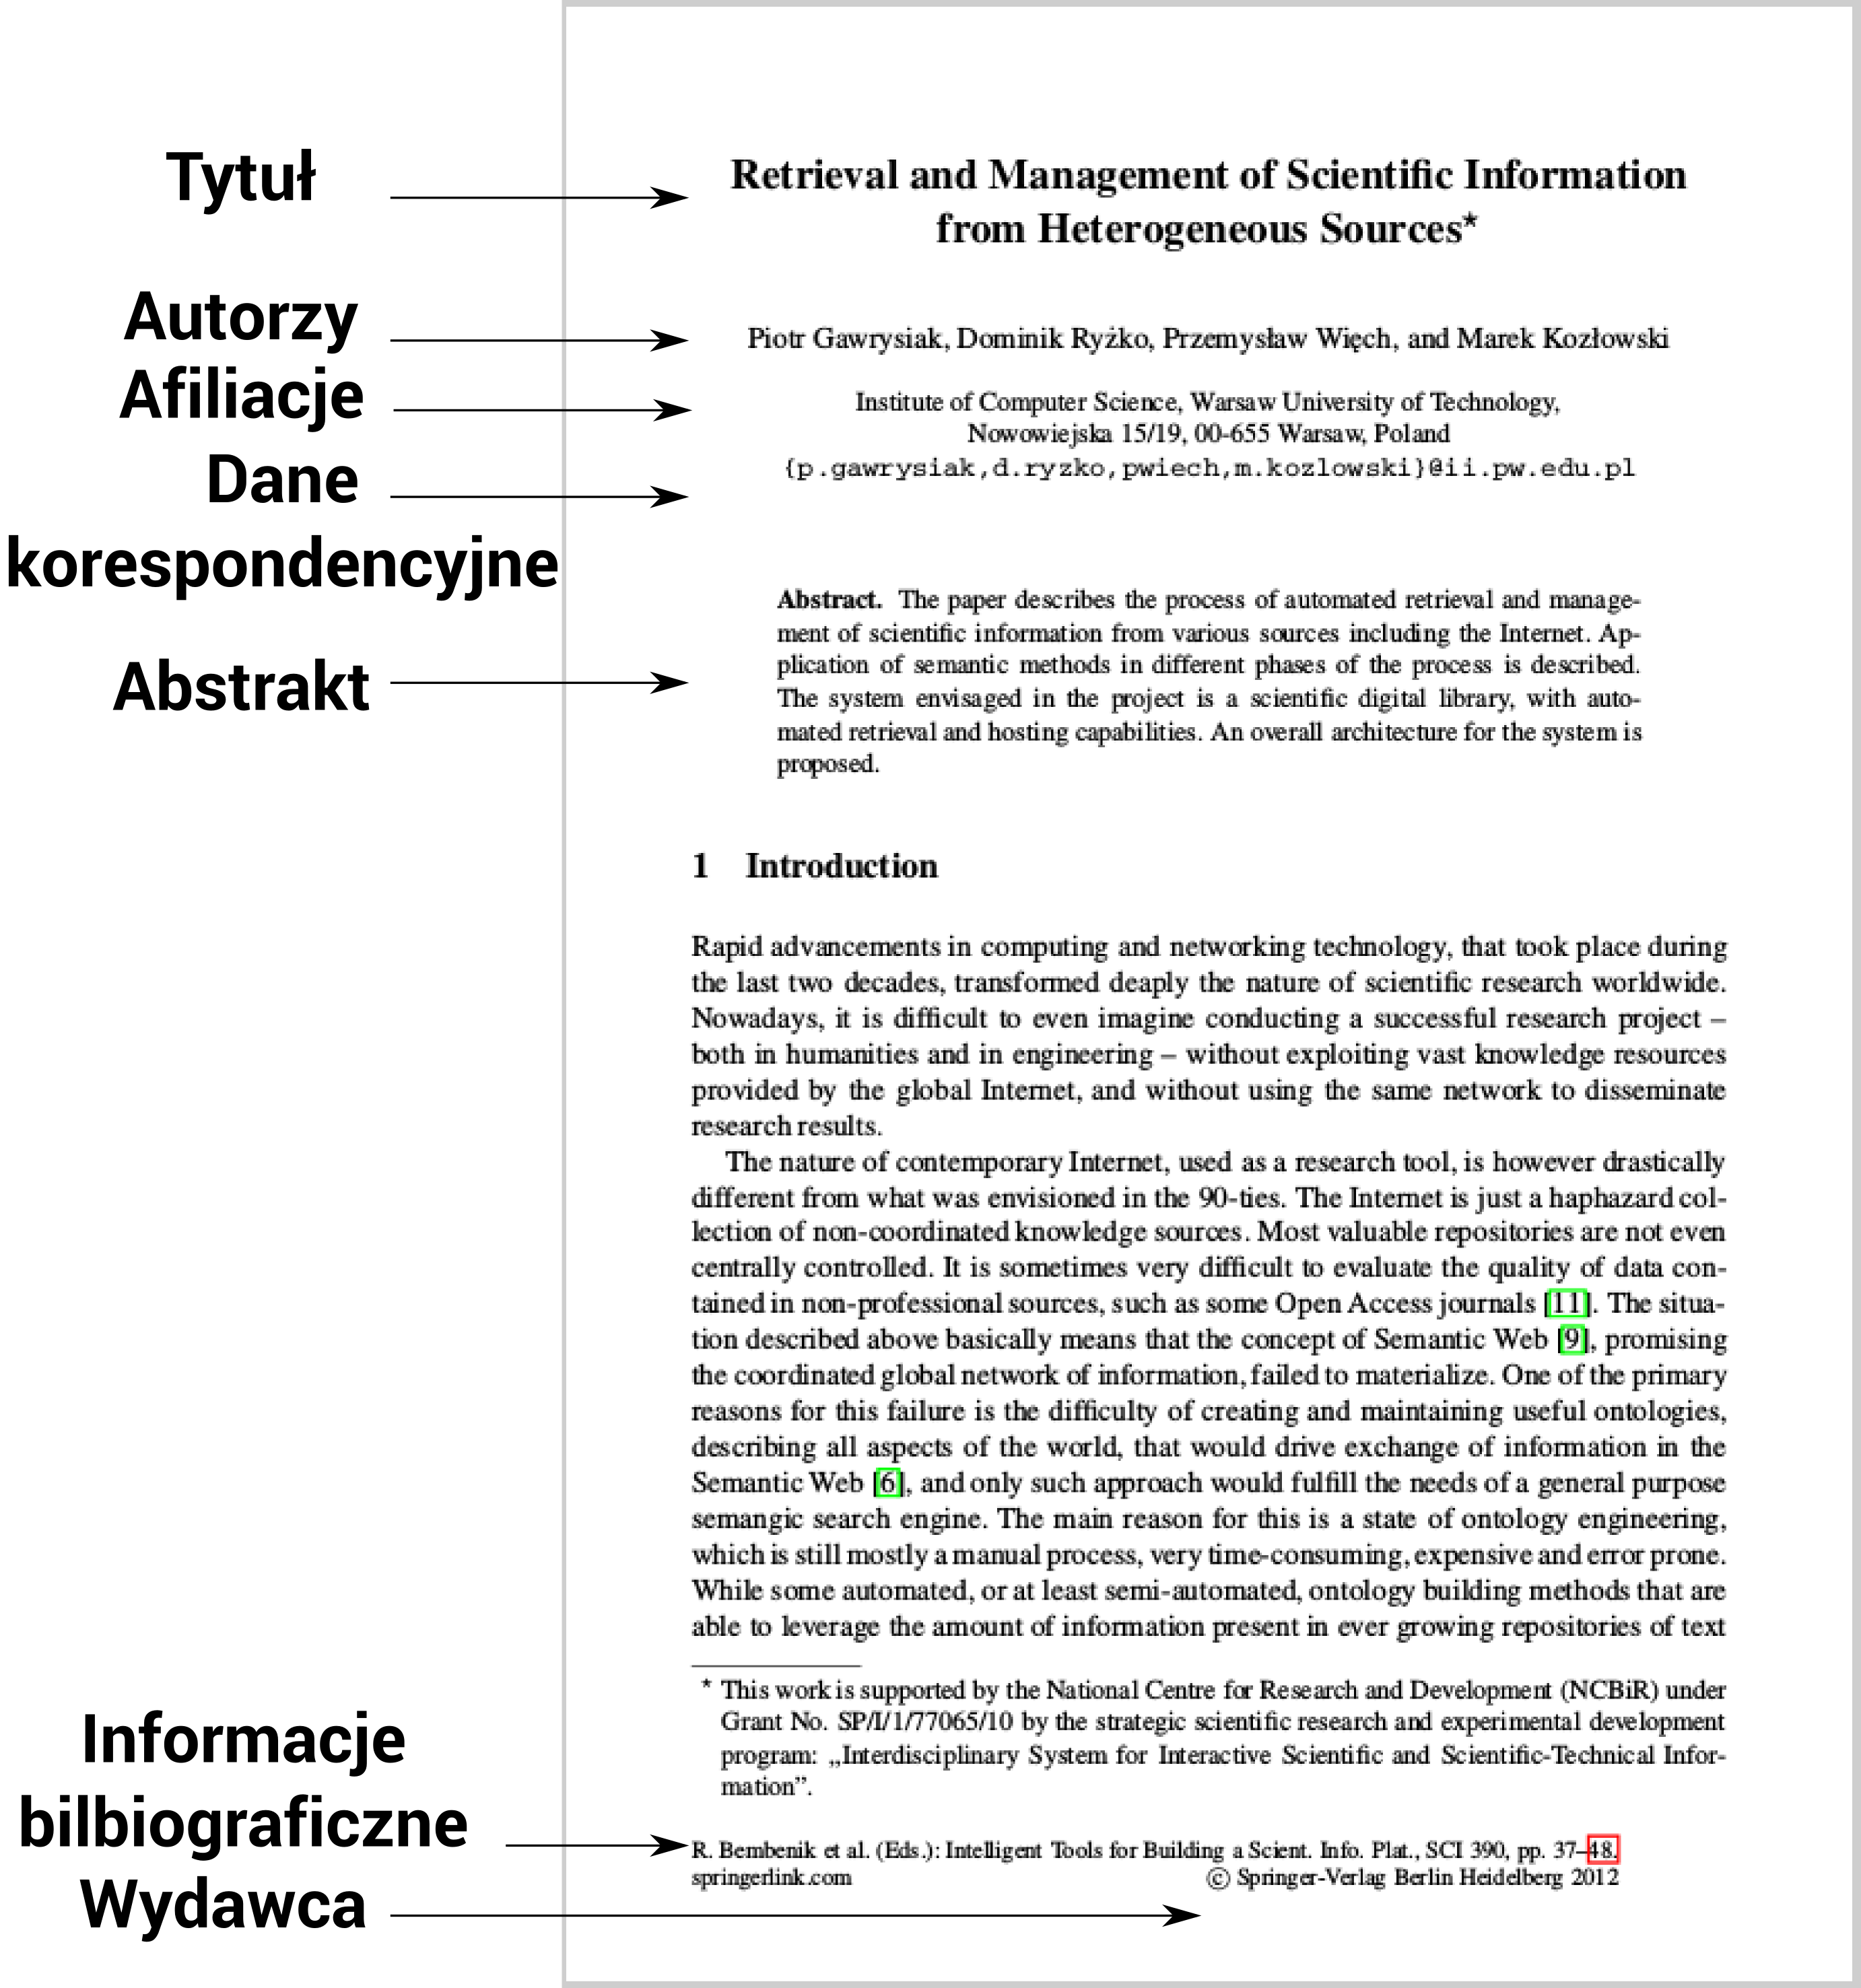
\includegraphics[width=0.9\textwidth]{art_meta.png}
\end{figure}
\column{.4\linewidth}
Dodatkowo:\\
\begin{itemize}
\item prawa kopiowania (ang. \textit{copyright}),
\item daty dostarczenia tekstu, edycji, publikacji,
\item edytor,
\item słowa kluczowe,
\item typ publikacji,
\item referencje bibliograficzne.
\end{itemize}
\end{columns}
\end{frame}
%%%%%%%%%%%%%%%%
\section{Etapy przetwarzania dokumentu}
\begin{frame}
\frametitle{Etapy przetwarzania dokumentu}
\begin{columns}
\column{.5\linewidth}
\begin{figure}[ht!]
  \centering
  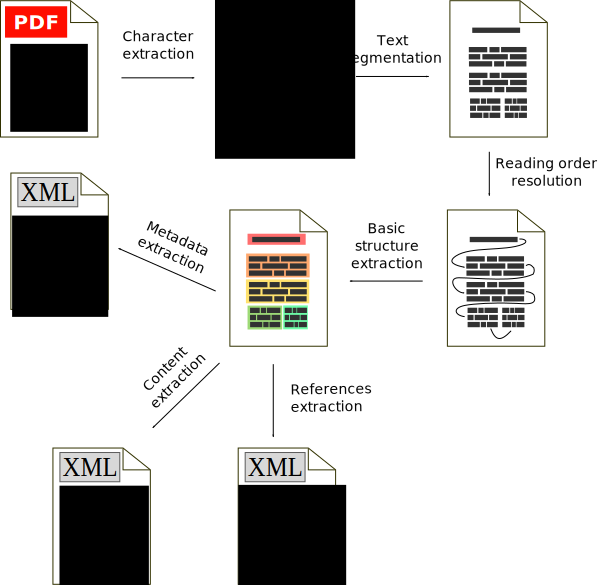
\includegraphics[width=6cm]{../graphics/pipeline}
  \label{fig:pipeline}
\end{figure}
\column{.5\textwidth}
\begin{enumerate}
\item ekstrakcja znaków z pliku
\item segmentacja tekstu
\item odtworzenie kolejności czytania
\item wstępna klasyfikacja bloków tesktu
\item przetwarzanie poszczególnych klas 
	\begin{enumerate}
		\item szczegółowa ekstrakcja metadanych
		\item ekstrakcja pełnego tekstu artykułu
		\item ekstrakcja referencji
	\end{enumerate}
\end{enumerate}
\end{columns}
\end{frame}
%%%%%%%%%%
\section{Klasyfikacja tekstu}
\begin{frame}
\frametitle{Maszyny wektorow wspierających (SVM)}
\begin{itemize}
\item<1-> algorytm klasyfikacji (uczenia z nadzorem)
\item<2-> uczenie polega na znalezieniu optymalnej (hiper-)płaszczyzny separującej zbiór punktów należących do dwóch klas decyzyjnych
\item<3-> klasyfikacja nieznanych punktów polega na określeniu po której stronie płaszczyzny decyzyjnej znajduje się dany punkt
\item<4-> jądro przekształcenia pozwala na przeniesienie punktów do przestrzeni o wyższej wymiarowości

\begin{center}
\begin{figure}
\centering
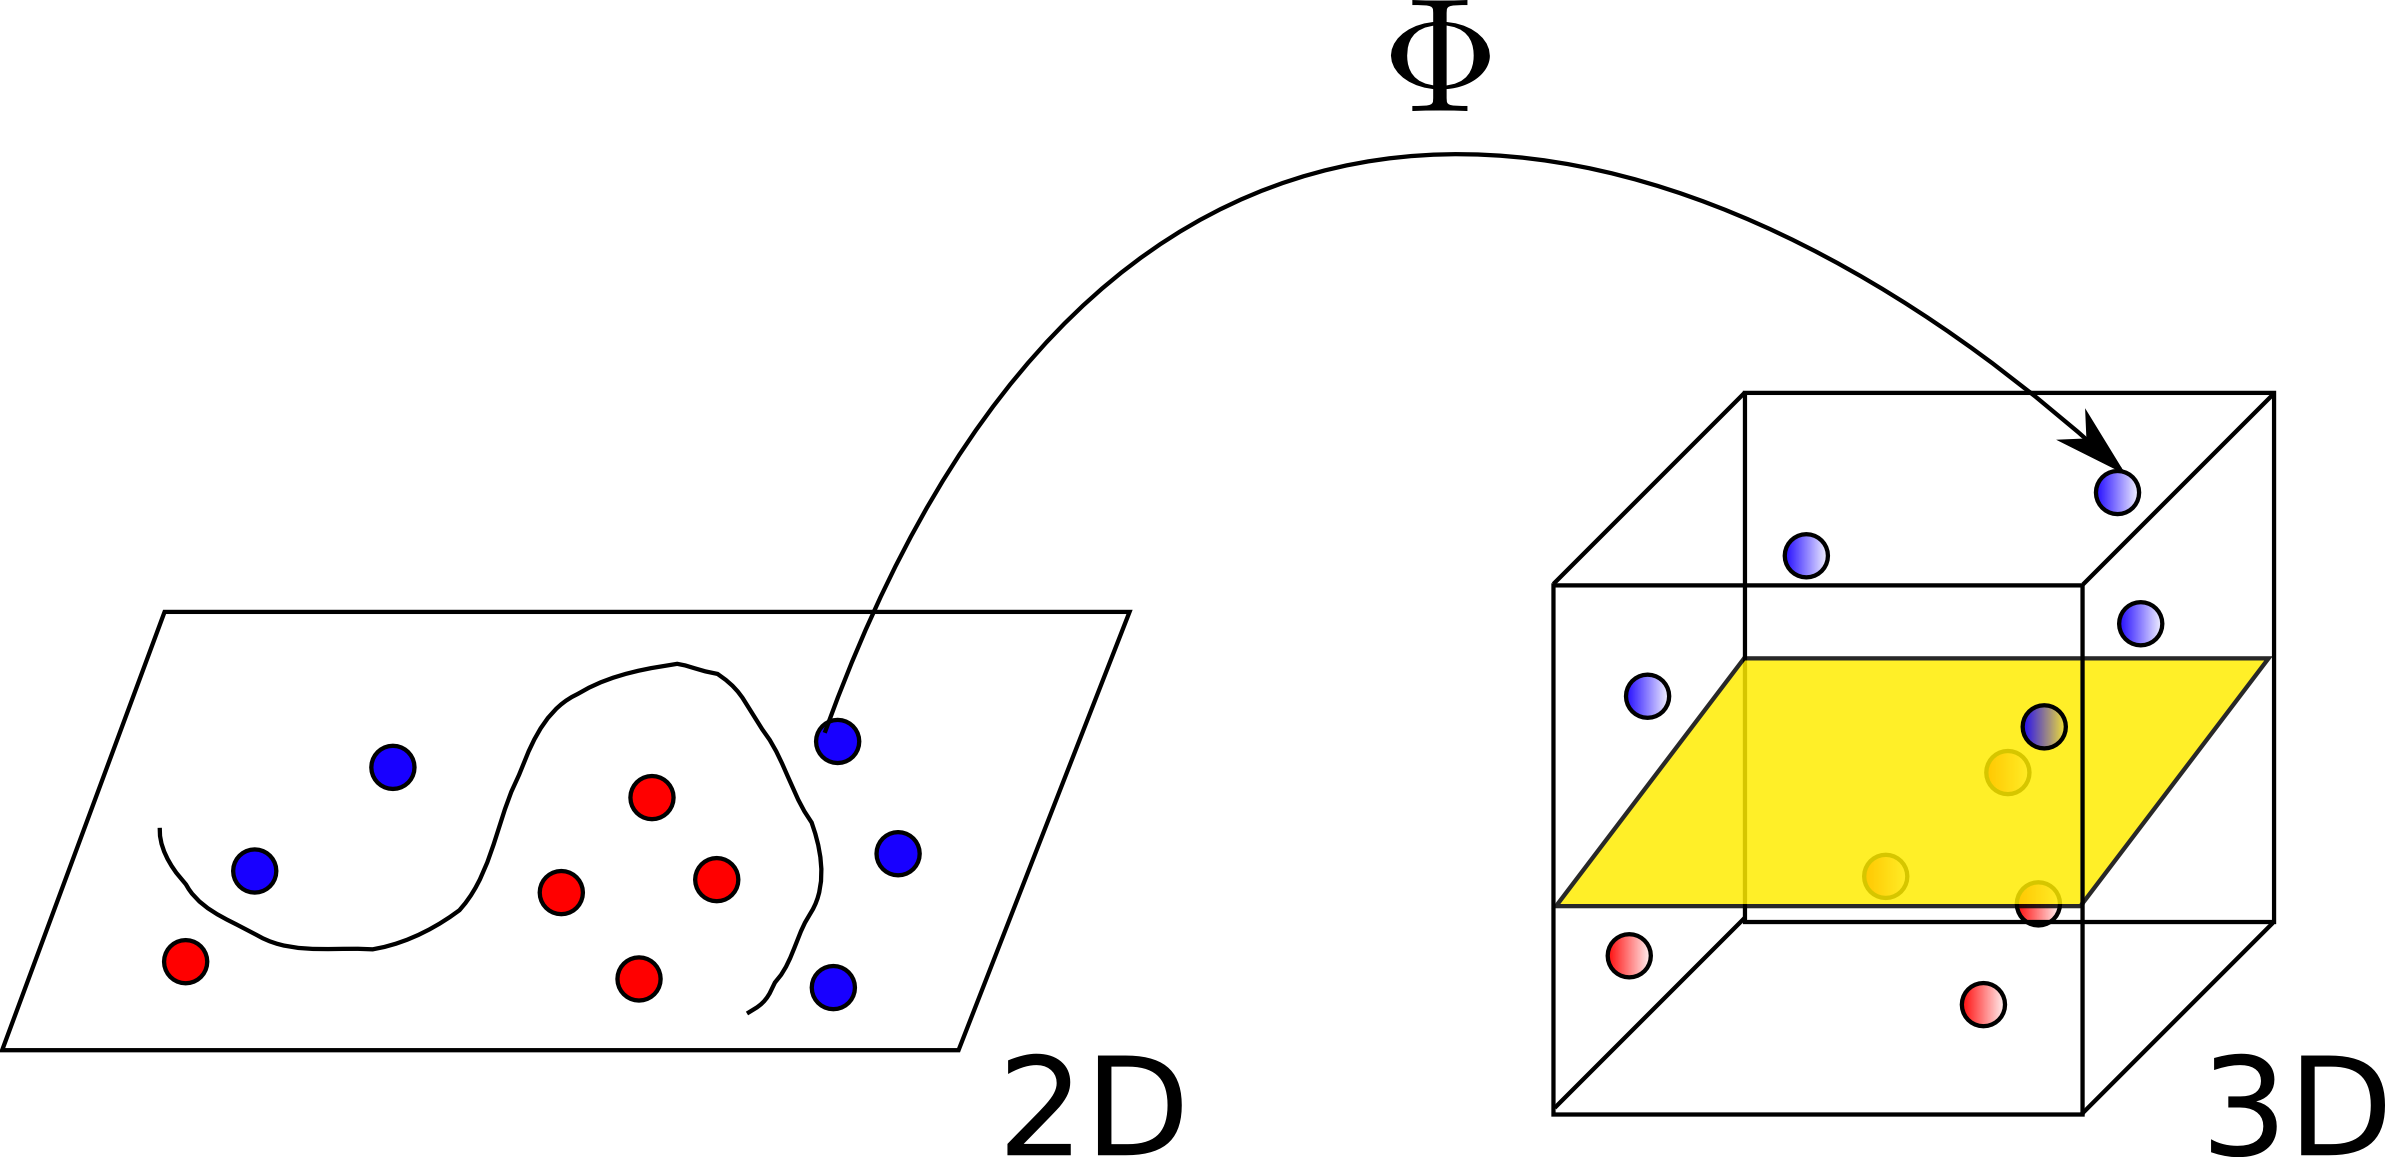
\includegraphics[width=4cm]{2dto3d.png}
\end{figure}
\end{center}
\item<5-> w pracy wykorzystano bibliotekę LibSVM
\end{itemize}
\end{frame}

%%%%%%%%%%%%%

\begin{frame}
\frametitle{Cechy klasyfikacyjne (ang. \protect{\textit{features}}) tekstu}
Klasyfikacja tekstu odbywa się per blok. Poniższe cechy są brane pod uwagę:
\begin{itemize}
\item Cechy formatowania
	\begin{itemize} \item Cechy użytych fontów, interlinii itp. \end{itemize}
\item Cechy układu
	\begin{itemize} \item Geometryczne cechy bloków tesktu: szerokość, wysokość, marginesy, odległość od innych bloków itp. 
	\item DistanceFromNearestNeighbourFeature
	\end{itemize}
\item Cechy semantyczne
	\begin{itemize} \item Zawartość predefiniowanych słów kluczowych (\textit{authors, email, abstract, keywords}, etc.) \end{itemize}
\item Cechy specjalne
\begin{itemize}\item klasa decyzyjna poprzedniego bloku tekstu \item \textit{IsAnywhereElseFeature} \item \textit{BracketCountFeature} \item \textit{CommaCountFeature} \end{itemize}
\end{itemize}
\end{frame}
%%%%%%%%%%
\begin{frame}
\frametitle{Strojenie systemu}
\begin{itemize}
\item System zawiera dwa klasyfikatory SVM, które przeprowadzają klasyfikację wstępną oraz szczegółową klasyfikację metadanych.
\item Optymalizacja polega na znalezieniu trójki $(K,C,\gamma)$, gdzie $K$ to jądro przekształcenia, $C$ to koszt nieprawidłowej klasyfikacji, a $\gamma$ to parametr przekształcenia.
\end{itemize}
\begin{columns}
\column{.5\textwidth}
\begin{figure}[]
  \centering
  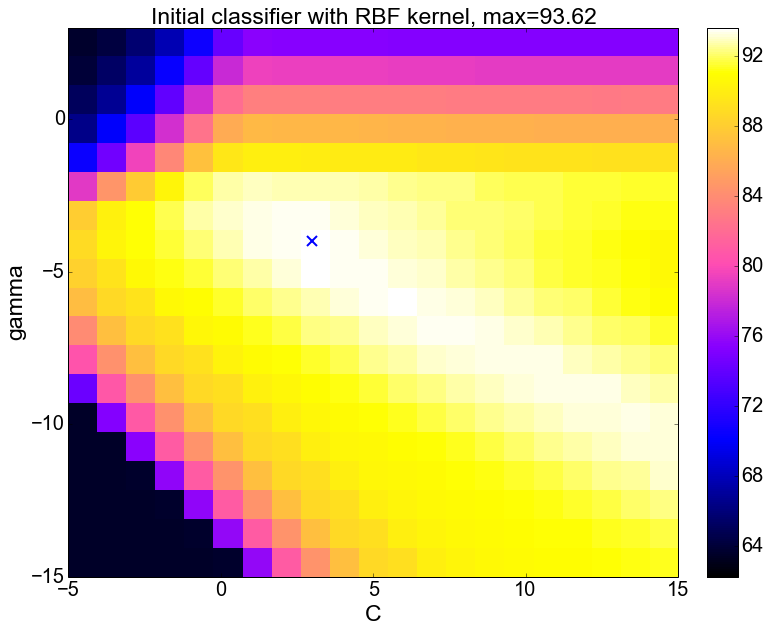
\includegraphics[width=4cm]{../plots/init_rbf.png}
  \label{fig:pipeline}
\end{figure}
\column{.5\textwidth}
\begin{figure}[]
  \centering
  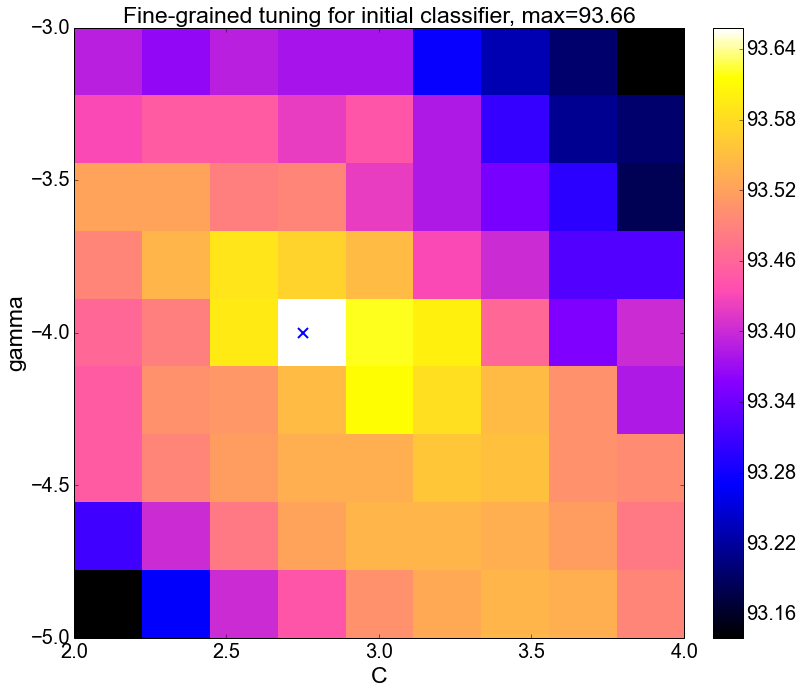
\includegraphics[width=4cm]{../plots/init_fine.png}
  \label{fig:pipeline}
\end{figure}
\end{columns}

\end{frame}


%%%%%%%%%%%
\section{GROTOAP2 - zbiór artykułów treningowych}
\begin{frame}
\frametitle{GROTOAP2 - zbiór artykułów treningowych}
\begin{itemize}
\item GROTOAP2 jest zbiorem 13,000 artykułów naukowych (pełne teksty w formacie PDF i dane \textit{Ground Truth} w formacie TrueViz) z kolekcji PUBMED. Artykuły pochodzą z 1170 czasopism od 208 wydawców,
\item Kolekcja PUBMED zawiera pełne teksty (PDF) oraz metadane (NLM) o różnych stopniu wiarygodności (z reguły zależne od czasopisma),
\item Metodologia tworzenia GROTOAP2:
\begin{enumerate}
\item Każdy artykuł z PUBMED został wstępnie przetworzony do formatu TrueViz
\item Metadane były dopasowywane do bloków tekstu przy użyciu dystansu Watermana-Smitha
\item Efekty dopasowywania były weryfikowane w procesie iteracyjnym (\textasciitilde 40). To pozwoliło na stworzenie reguł heurystycznych poprawiających odkryte nieprawidłowości.
\end{enumerate}

\end{itemize}

\end{frame}

%%%%%%%%%%%
\section{Ewaluacja}
\begin{frame}
\frametitle{Ewaluacja}
Ewaluacja systemu została oparta na 5-krotnej walidacji skrośnej przy użyciu GROTOAP2
\begin{table}[]
\renewcommand{\arraystretch}{1.5}
\centering
\tiny
\begin{tabular}{|r|c|c|c|c||c|c|}
\hline
& \rotatebox{90}{\textbf{BODY}} & \rotatebox{90}{\textbf{METADATA}} & \rotatebox{90}{\textbf{REFERENCES }} & \rotatebox{90}{\textbf{OTHER}} & \rotatebox{90}{\textbf{precyzja}} & \rotatebox{90}{\textbf{kompletność}} \\ \hline \hline
\textbf{BODY} & \textbf{167467} & 1394 & 350 & 769 & 96.95 & 98.52 \\ \hline
\textbf{METADATA} & 2094 & \textbf{51707} & 52 & 392 & 95.99 & 95.32  \\ \hline
\textbf{REFERENCES} & 1457 & 45 & \textbf{9641} & 97 & 95.67 & 87.77 \\ \hline
\textbf{OTHER} & 1724 & 719 & 34 & \textbf{24202}& 95.06 & 90.72 \\ \hline
\end{tabular}
% \caption{Macierz konfuzji dla klasyfikacji wstępnej.}
\label{tab:initial_confusion_matrix}
\end{table}
\begin{table}\centering\tiny
% \floatbox[{\capbeside\thisfloatsetup{capbesideposition={right,top},capbesidewidth=4cm}}]
% {\caption{A test figure with its caption side by side}}
\setlength{\tabcolsep}{3pt}
\renewcommand{\arraystretch}{1.5}
\begin{tabular}{|r|c|c|c|c|c|c|c|c|c|c|c|c|}

\hline% \parbox[b]{\hsize}
& \rotatebox{90}{\textbf{abstract}} & \rotatebox{90}{\textbf{affiliation}} & \rotatebox{90}{\textbf{author}} & \rotatebox{90}{\textbf{bib\_info}} & \rotatebox{90}{\textbf{copyright}} & \rotatebox{90}{\textbf{correspondence}} & \rotatebox{90}{\textbf{dates}} & \rotatebox{90}{\textbf{editor}} & \rotatebox{90}{\textbf{keywords}} & \rotatebox{90}{\textbf{title}} & \rotatebox{90}{\textbf{title\_author}} & \rotatebox{90}{\textbf{type}} \\
\hline
precyzja  & 98.18 & 95.55 & 97.71 & 97.62 & 95.72 & 90.04 & 97.15 & 98.69 & 93.67 & 98.61 & 96.53 & 93.73 \\ \hline
kompletność  & 97.96 & 97.76 & 94.46 & 99.05 & 92.58 & 89.38 & 92.16 & 98.22 & 80.70 & 98.74 & 96.0 & 87.74 \\ \hline
\end{tabular}
\end{table}
\end{frame}
%%%%%%%%%%%%
\section{Przyszła praca}
\begin{frame}
\frametitle{Przyszła praca}
Działanie systemu może być poprawione poprzez:
\begin{itemize}
\item optymalizacja klasyfikatora poprzez zaaplikowanie zbioru algorytmów (np. WEKA, scikit-learn) i wybór globalnie najefektywniejszego,
\item poprawienie pokrycia bloków tekstu w zbiorze GROTOAP2,
\item systematyczna optymalizacja algorytmu segmentacji,
\item dokładne parsowanie nazwisk autorów (pierwsze i drugie imię, nazwisko),
\end{itemize}
\end{frame}
%%%%%%%%%%%%
\begin{frame}
\frametitle{Demonstracja}
\end{frame}
%%%%%%%%%%%%%
\begin{frame}
\frametitle{Slajdy zapasowe - publikacje}
\centering
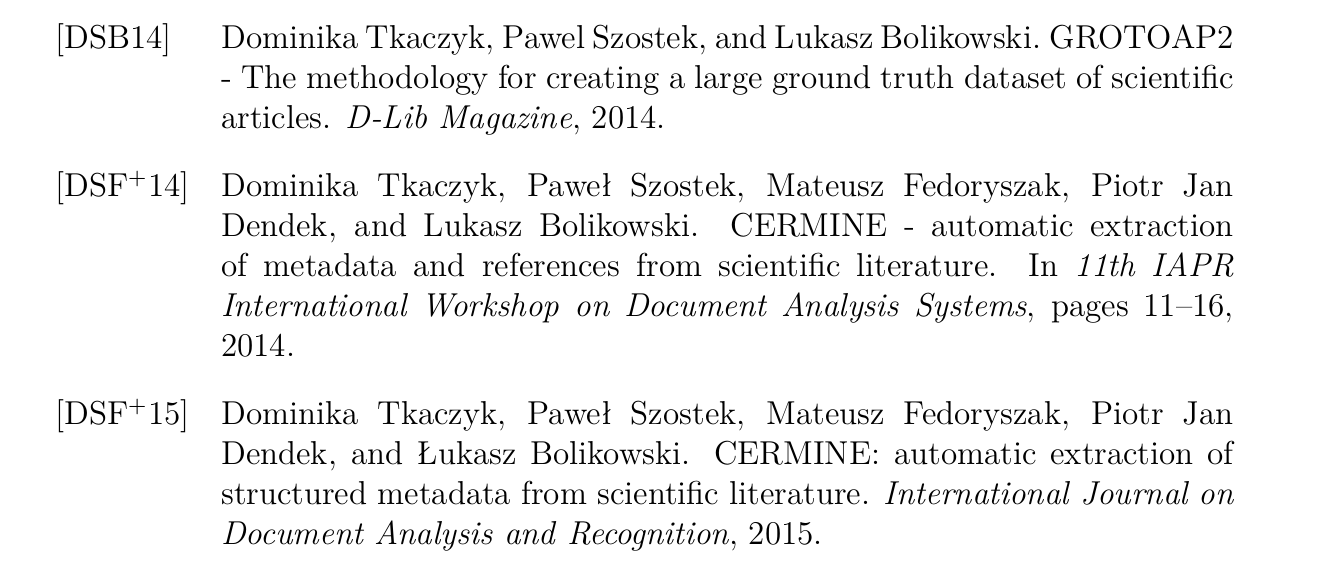
\includegraphics[width=10cm]{cit.png}

\end{frame}
\end{document}